\setcounter{section}{22}
\setcounter{subsection}{8}
\setcounter{subsubsection}{0}
% Copyright 2019 by Till Tantau
%
% This file may be distributed and/or modified
%
% 1. under the LaTeX Project Public License and/or
% 2. under the GNU Free Documentation License.
%
% See the file doc/generic/pgf/licenses/LICENSE for more details.


\section{Transparency\\透明度}
\label{section-tikz-transparency}

\subsection{Overview\\概述}

Normally, when you paint something using any of \tikzname's commands (this
includes stroking, filling, shading, patterns, and images), the newly painted
objects totally obscure whatever was painted earlier in the same area.

通常,当您使用 \tikzname\ 的任何绘图命令(包括描边、填充、着色、图案和图像)绘制某些内容时,新绘制的对象会完全遮挡先前在同一区域绘制的内容。

You can change this behavior by using something that can be thought of as
``(semi)transparent colors''. Such colors do not completely obscure the
background, rather they blend the background with the new color. At first
sight, using such semitransparent colors might seem quite straightforward, but
the math going on in the background is quite involved and the correct handling
of transparency fills some 64 pages in the PDF specification.

您可以通过使用可以被视为“(半)透明颜色”的东西来改变这种行为。这种颜色不会完全遮挡背景,而是将背景与新颜色混合在一起。乍一看,使用这种半透明颜色可能看起来很简单,但背后进行的数学计算非常复杂,正确处理透明度需要填充大约 64 页的 PDF 规范。

In the present section, we start with the different ways of specifying ``how
transparent'' newly drawn objects should be. The simplest way is to just
specify a percentage like ``60\% transparent''. A much more general way is to
use something that I call a \emph{fading}, also known as a soft mask or a mask.

在本节中,我们首先介绍了指定新绘制对象的“透明程度”的不同方法。最简单的方法是仅指定一个百分比,如“60\% 的透明度”。更通用的方法是使用我称之为“渐变”(fading)的东西,也称为软蒙版或蒙版。

At the end of the section we address the problem of creating so-called
\emph{transparency groups}. This problem arises when you paint over a position
several times with a semitransparent color. Sometimes you want the effect to
accumulate, sometimes you do not.

在本节的最后,我们解决了创建所谓的“透明组”(transparency groups)的问题。当您多次在同一位置使用半透明颜色进行绘制时,就会出现此问题。有时您希望效果累积,有时则不希望。

\emph{Note:} Transparency (or Opacity, as it may be called as well) is best
supported by the pdf\TeX\ driver. The \textsc{svg} driver also has some
support. The PostScript file format does not know about transparency. In
|dvips|-generated PostScript files, transparency of graphic objects is defined
through special commands that need further processing to become visible in the
\textsc{pdf} output. For this, a recent version of Ghostscript, preferably 9.52
or newer, is required and its command line utility |ps2pdf| must be called with
option |-dALLOWPSTRANSPARENCY|. Older versions may need option |-dNOSAFER|
instead, but some advanced features, such as \emph{transparency groups} and
\emph{fadings}, may not work at all. Printers and other programs will typically
ignore opacity settings in PostScript files.

\emph{注意:}透明度(也称为不透明度)在 pdf\TeX\ 驱动程序中得到最好的支持。\textsc{svg} 驱动程序也具有一些支持。PostScript 文件格式不支持透明度。在由 |dvips| 生成的 PostScript 文件中,图形对象的透明度是通过特殊命令定义的,这些命令需要进一步处理才能在 \textsc{pdf} 输出中显示。为此,需要使用 Ghostscript 的最新版本,最好是 9.52 或更新版本,并且必须使用其命令行实用程序 |ps2pdf| 并带有选项 |-dALLOWPSTRANSPARENCY|。较旧的版本可能需要选项 |-dNOSAFER|,但某些高级功能(例如“透明组”和“渐变”)可能根本无法正常工作。打印机和其他程序通常会忽略 PostScript 文件中的不透明度设置。


\subsection{Specifying a Uniform Opacity\\指定统一的不透明度}

Specifying a stroke and/or fill opacity is quite easy using the following
options.

使用以下选项可以很容易地指定描边和/或填充的不透明度。

\begin{key}{/tikz/draw opacity=\meta{value}}
    This option sets ``how transparent'' lines should be. A value of |1| means
    ``fully opaque'' or ``not transparent at all'', a value of |0| means
    ``fully transparent'' or ``invisible''. A value of |0.5| yields lines that
    are semitransparent.

    此选项设置线条的“透明程度”。值 |1| 表示“完全不透明”或“完全不透明”,值 |0| 表示“完全透明”或“不可见”。值 |0.5| 会产生半透明线条。

    Note that when you use PostScript as your output format, this option works
    only with recent versions of Ghostscript.
    
    请注意,当您使用 PostScript 作为输出格式时,此选项仅适用于 Ghostscript 的最新版本。
\begin{codeexample}[]
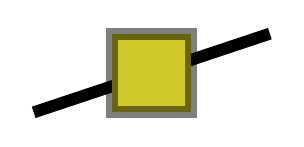
\begin{tikzpicture}[line width=1ex]
  \draw (0,0) -- (3,1);
  \filldraw [fill=yellow!80!black,draw opacity=0.5] (1,0) rectangle (2,1);
\end{tikzpicture}
\end{codeexample}
    %
\end{key}

Note that the |draw opacity| options only sets the opacity of drawn lines. The
opacity of fillings is set using the option |fill opacity| (documented in
Section~\ref{section-fill-opacity}. The option |opacity| sets both at the same
time.

请注意,|draw opacity|选项仅设置绘制线条的不透明度。填充的不透明度使用|fill opacity|选项设置(在第~\ref{section-fill-opacity}节中有文档记录)。|opacity|选项同时设置两者。

\begin{key}{/tikz/opacity=\meta{value}}
    Sets both the drawing and filling opacity to \meta{value}.

    将绘制和填充的不透明度都设置为\meta{value}。

    The following predefined styles make it easier to use this option:

    下面的预定义样式使使用此选项更加容易:
    %
    \begin{stylekey}{/tikz/transparent}
        Makes everything totally transparent and, hence, invisible.
        
        使所有内容完全透明,因此不可见。


\begin{codeexample}[]
\tikz{\fill[red]             (0,0)   rectangle (1,0.5);
      \fill[transparent,red] (0.5,0) rectangle (1.5,0.25); }
\end{codeexample}
    \end{stylekey}

    \begin{stylekey}{/tikz/ultra nearly transparent}
        Makes everything, well, ultra nearly transparent.
        
        使所有内容几乎完全透明。
\begin{codeexample}[]
\tikz{\fill[red]                      (0,0)   rectangle (1,0.5);
      \fill[ultra nearly transparent] (0.5,0) rectangle (1.5,0.25); }
\end{codeexample}
    \end{stylekey}

    \begin{stylekey}{/tikz/very nearly transparent}
\begin{codeexample}[]
\tikz{\fill[red]                     (0,0)   rectangle (1,0.5);
      \fill[very nearly transparent] (0.5,0) rectangle (1.5,0.25); }
\end{codeexample}
    \end{stylekey}

    \begin{stylekey}{/tikz/nearly transparent}
\begin{codeexample}[]
\tikz{\fill[red]                (0,0)   rectangle (1,0.5);
      \fill[nearly transparent] (0.5,0) rectangle (1.5,0.25); }
\end{codeexample}
    \end{stylekey}

    \begin{stylekey}{/tikz/semitransparent}
\begin{codeexample}[]
\tikz{\fill[red]             (0,0)   rectangle (1,0.5);
      \fill[semitransparent] (0.5,0) rectangle (1.5,0.25); }
\end{codeexample}
    \end{stylekey}

    \begin{stylekey}{/tikz/nearly opaque}
\begin{codeexample}[]
\tikz{\fill[red]           (0,0)   rectangle (1,0.5);
      \fill[nearly opaque] (0.5,0) rectangle (1.5,0.25); }
\end{codeexample}
    \end{stylekey}

    \begin{stylekey}{/tikz/very nearly opaque}
\begin{codeexample}[]
\tikz{\fill[red]                (0,0)   rectangle (1,0.5);
      \fill[very nearly opaque] (0.5,0) rectangle (1.5,0.25); }
\end{codeexample}
    \end{stylekey}

    \begin{stylekey}{/tikz/ultra nearly opaque}
\begin{codeexample}[]
\tikz{\fill[red]                 (0,0)   rectangle (1,0.5);
      \fill[ultra nearly opaque] (0.5,0) rectangle (1.5,0.25); }
\end{codeexample}
    \end{stylekey}

    \begin{stylekey}{/tikz/opaque}
        This yields completely opaque drawings, which is the default.
        
        这将产生完全不透明的绘图,这是默认设置。

\begin{codeexample}[]
\tikz{\fill[red]    (0,0)   rectangle (1,0.5);
      \fill[opaque] (0.5,0) rectangle (1.5,0.25); }
\end{codeexample}
    \end{stylekey}
\end{key}

\begin{key}{/tikz/fill opacity=\meta{value}}
    This option sets the opacity of fillings. In addition to filling
    operations, this opacity also applies to text and images.

    此选项设置填充的不透明度。除了填充操作外,此不透明度还适用于文本和图像。

    Note, again, that when you use PostScript as your output format, this
    option works only with recent versions of Ghostscript.

    请再次注意,当将PostScript作为输出格式时,此选项仅适用于最新版本的Ghostscript。
    %
\begin{codeexample}[]
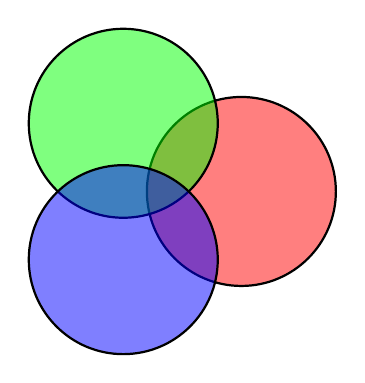
\begin{tikzpicture}[thick,fill opacity=0.5]
  \filldraw[fill=red]   (0:1cm)    circle (12mm);
  \filldraw[fill=green] (120:1cm)  circle (12mm);
  \filldraw[fill=blue]  (-120:1cm) circle (12mm);
\end{tikzpicture}
\end{codeexample}

\begin{codeexample}[]
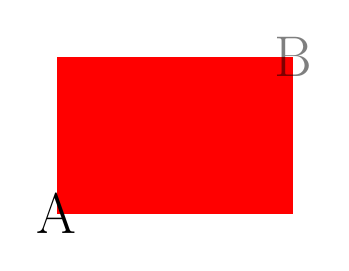
\begin{tikzpicture}
  \fill[red] (0,0) rectangle (3,2);

  \node                   at (0,0) {\huge A};
  \node[fill opacity=0.5] at (3,2) {\huge B};
\end{tikzpicture}
\end{codeexample}
    %
\end{key}

\begin{key}{/tikz/text opacity=\meta{value}}
    Sets the opacity of text labels, overriding the |fill opacity| setting.
    
    设置文本标签的不透明度,覆盖|fill opacity|设置。

\begin{codeexample}[]
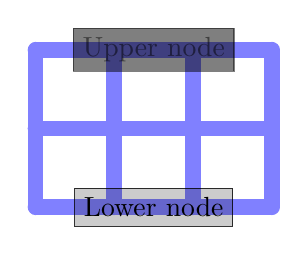
\begin{tikzpicture}[every node/.style={fill,draw}]
  \draw[line width=2mm,blue!50,line cap=round] (0,0) grid (3,2);

  \node[opacity=0.5] at (1.5,2) {Upper node};
  \node[draw opacity=0.8,fill opacity=0.2,text opacity=1]
    at (1.5,0) {Lower node};
\end{tikzpicture}
\end{codeexample}
    %
\end{key}

Note the following effect: If you set up a certain opacity for stroking or
filling and you stroke or fill the same area twice, the effect accumulates:

请注意以下效果:如果您为描边或填充设置一定的不透明度,并且两次描边或填充相同的区域,则效果会累积:


\begin{codeexample}[]
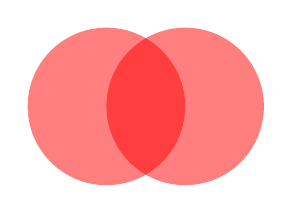
\begin{tikzpicture}[fill opacity=0.5]
  \fill[red] (0,0) circle (1);
  \fill[red] (1,0) circle (1);
\end{tikzpicture}
\end{codeexample}

Often, this is exactly what you intend, but not always. You can use
transparency groups, see the end of this section, to change this.

通常,这正是您想要的效果,但并非总是如此。您可以使用透明度组(见本节末尾)来改变这种情况。


\subsection{Blend Modes\\混合模式}
\label{section-blend-modes}

A \emph{blend mode} specifies how colors mix when you paint on a canvas.
Normally, if you paint a red box on a green circle, the red color will
completely replace the green circle. However, in some situations you might also
wish the red color to somehow ``mix'' or ``blend'' with the green circle. We
already saw that, using transparency, we can draw something without completely
obscuring the background. \emph{Blending} is a similar operation, only here we
mix colors in more complicated ways.

\emph{混合模式}指定在画布上绘制时颜色如何混合。通常,如果您在绿色圆上绘制一个红色框,红色将完全替换绿色圆。然而,在某些情况下,您可能还希望红色与绿色圆以某种方式“混合”或“融合”。我们已经看到,使用透明度,我们可以在不完全遮挡背景的情况下绘制某些内容。而\emph{混合}是一种类似的操作,只是这里我们以更复杂的方式混合颜色。

\emph{Note:} Blending is a rather ``advanced'' feature of \textsc{pdf}. Most
renderers, let alone printers, will have trouble rendering blending correctly.

\emph{注意:}混合是\textsc{pdf}的一个相对“高级”的功能。大多数渲染器,更不用说打印机了,都难以正确渲染混合效果。

\begin{key}{/tikz/blend mode=\meta{mode}}
    Sets the current blend mode to \meta{mode}. Here \meta{mode} must be one of
    the modes listed below. More details on these modes can also be found in
    Section~7.2.4 of the \textsc{pdf} Specification, version~1.7.

    将当前混合模式设置为\meta{mode}。这里\meta{mode}必须是下面列出的模式之一。关于这些模式的更多详细信息也可以在\textsc{pdf}规范版本1.7的第7.2.4节中找到。

    In the following example, the blend mode is only used and set inside a
    transparency group (see also Section~\ref{section-transparency-groups}).
    This is because most renderers (viewing programs) have trouble rendering
    blending correctly otherwise. For instance, at the time of writing, the
    versions of Adobe's Reader and Apple's Preview render the following drawing
    very differently, if the transparency group is not used in the following
    example.
    
    在以下示例中,混合模式仅在透明度组内部使用和设置(另请参见第\ref{section-transparency-groups}节)。这是因为大多数渲染器(查看程序)在没有使用透明度组的情况下难以正确渲染混合效果。例如,在撰写本文时,Adobe Reader和Apple Preview的版本在未在以下示例中使用透明度组时,会以非常不同的方式渲染以下绘图。


\begin{codeexample}[]
\tikz {
  \begin{scope}[transparency group]
    \begin{scope}[blend mode=screen]
      \fill[red!90!black]   ( 90:.6) circle (1);
      \fill[green!80!black] (210:.6) circle (1);
      \fill[blue!90!black]  (330:.6) circle (1);
    \end{scope}
  \end{scope}
}
\end{codeexample}

    Because of the trouble with rendering blending correctly outside
    transparency groups, there is a special key that establishes a transparency
    group and sets a blend mode simultaneously:

    由于在透明度组之外正确渲染混合效果存在问题,因此有一个特殊的键可以同时建立透明度组并设置混合模式:

    \begin{key}{/tikz/blend group=\meta{mode}}
        This key can only be used with a scope (like |transparency group|). It
        will cause the current scope to become a transparency group and, inside
        this group, the blend mode will be set to \meta{mode}.

        此键只能与作用域(如|transparency group|)一起使用。它将导致当前作用域成为透明度组,并且在该组内部,混合模式将设置为\meta{mode}。

        %
\begin{codeexample}[]
\tikz [blend group=screen] {
  \fill[red!90!black]   ( 90:.6) circle (1);
  \fill[green!80!black] (210:.6) circle (1);
  \fill[blue!90!black]  (330:.6) circle (1);
}
\end{codeexample}
    \end{key}

    Here is an overview of the effects of the different available blend modes.
    In the examples, we always have three circles drawn on top of each other
    (as in the example code earlier): We start with a triple of pure red,
    green, and blue. Below it, we have a triple of light versions of these
    three colors (|red!50|, |green!50|, and |blue!50|). Next comes the triple
    yellow, cyan, and magenta; again with a triple of light versions below it.
    The large example consists of three balls (produced using |ball color|)
    having the colors red, green, and blue, are drawn on top of each other just
    like the circles.

    下面是不同可用混合模式的效果概述。在示例中,我们始终有三个互相叠加的圆(与前面的示例代码中的情况相同):我们从纯红、绿、蓝的三重组合开始。在其下方,我们有这三种颜色的浅色版本(|red!50|、|green!50|和|blue!50|)。接下来是黄色、青色和洋红色的三重组合,再次在其下方有三种颜色的浅色版本。大型示例由三个球(使用|ball color|生成)组成,颜色分别为红色、绿色和蓝色,与圆形一样叠加绘制。

    \definecolor{rg}{rgb}{1,1,0}
    \definecolor{gb}{rgb}{0,1,1}
    \definecolor{br}{rgb}{1,0,1}

    \def\makeline#1#2#3{\leavevmode
        \hbox to 40mm{#1\hss}\ \hbox to
        20.5mm{#2\hss}\ \begin{minipage}[t]{88.5mm}\raggedright#3\end{minipage}\par
        \textcolor{black!25}{\hrule height1pt}
    }

    \def\showmode#1#2{
        \makeline{
            \tikz [blend mode=#1,baseline=-.5ex] {
              \fill[red]      ( 90:.5em) circle (.75em);
              \fill[green]    (210:.5em) circle (.75em);
              \fill[blue]     (330:.5em) circle (.75em);
              \scoped[yshift=-2.5em]{
                \fill[red!50]   ( 90:.5em) circle (.75em);
                \fill[green!50] (210:.5em) circle (.75em);
                \fill[blue!50]  (330:.5em) circle (.75em);
              }
            }
            \tikz [blend mode=#1,baseline=-.5ex] {
              \fill[rg]       ( 90:.5em) circle (.75em);
              \fill[gb]       (210:.5em) circle (.75em);
              \fill[br]       (330:.5em) circle (.75em);
              \scoped[yshift=-2.5em]{
                \fill[rg!50]  ( 90:.5em) circle (.75em);
                \fill[gb!50]  (210:.5em) circle (.75em);
                \fill[br!50]  (330:.5em) circle (.75em);
              }
            }
            \tikz [blend mode=#1,baseline=-.5ex+1.25em] {
              \shade[ball color=red]   ( 90:1em) circle (1.5em);
              \shade[ball color=green] (210:1em) circle (1.5em);
              \shade[ball color=blue]  (330:1em) circle (1.5em);
            }}{\verb|#1|}{#2}%
               % this argument was changed from {|#1|}  这个参数从{|#1|}改变
               % --> see <https://sourceforge.net/p/pgf/bugs/486/> --> 请参见https://sourceforge.net/p/pgf/bugs/486/
    } 

    \medskip
    \makeline{\emph{Example}}{\emph{Mode}}{\emph{Explanations quoted from
        Table~7.2 of the \textsc{pdf} Specification, Version~1.7}}

        \makeline{\emph{示例}}{\emph{模式}}{\emph{引用自\textsc{pdf}规范版本1.7的表7.2的解释}}
    \showmode{normal}{When painting a pixel with a some color (called the
        ``source color''), the background color (called the ``backdrop'') is
        completely ignored.}

        \showmode{normal}{当使用某种颜色(称为“源颜色”)绘制像素时,背景颜色(称为“背景”)完全被忽略。}

    \showmode{multiply}{Multiplies the backdrop and source color values. The
        result color is always at least as dark as either of the two
        constituent colors. Multiplying any color with black produces black;
        multiplying with white leaves the original color unchanged. Painting
        successive overlapping objects with a color other than black or white
        produces progressively darker colors.}

        \showmode{multiply}{将背景颜色和源颜色值相乘。结果颜色始终至少与两个组成颜色中的任何一个一样深。将任何颜色与黑色相乘会产生黑色;与白色相乘不会改变原始颜色。使用除黑色或白色以外的颜色连续叠加绘制对象会产生逐渐变暗的颜色。}

    \showmode{screen}{Multiplies the complements of the backdrop and source
        color values, then complements the result. The result color is always
        at least as light as either of the two constituent colors. Screening
        any color with white produces white; screening with black leaves the
        original color unchanged. The effect is similar to projecting multiple
        photographic slides simultaneously onto a single screen.}

        \showmode{screen}{将背景颜色的补和源颜色的补相乘,然后再取补。结果颜色始终至少与两个组成颜色中的任何一个一样亮。将任何颜色与白色相乘会产生白色;与黑色相乘不会改变原始颜色。效果类似于同时将多个幻灯片投影到一个屏幕上。}

    \showmode{overlay}{Multiplies or screens the colors, depending on the
        backdrop color value. Source colors overlay the backdrop while
        preserving its highlights and shadows. The backdrop color is not
        replaced but is mixed with the source color to reflect the lightness or
        darkness of the backdrop.}

        \showmode{overlay}{根据背景颜色值,将源颜色覆盖在背景上,同时保留其高光和阴影。背景颜色不被替换,而是与源颜色混合,以反映背景的亮度或暗度。}

    \showmode{darken}{Selects the darker of the backdrop and source colors. The
        backdrop is replaced with the source where the source is darker;
        otherwise, it is left unchanged.}

        \showmode{darken}{选择较暗的背景颜色和源颜色。如果源颜色较暗,则用源颜色替换背景;否则,保持不变。}

    \showmode{lighten}{Selects the lighter of the backdrop and source colors.
        The backdrop is replaced with the source where the source is lighter;
        otherwise, it is left unchanged.}

        \showmode{lighten}{选择较亮的背景颜色和源颜色。如果源颜色较亮,则用源颜色替换背景;否则,保持不变。}

    \showmode{color dodge}{Brightens the backdrop color to reflect the source
        color. Painting with black produces no changes.}

        \showmode{color dodge}{增亮背景颜色以反映源颜色。使用黑色绘制不会产生变化。}

    \showmode{color burn}{Darkens the backdrop color to reflect the source
        color. Painting with white produces no change.}

        \showmode{color burn}{变暗背景颜色以反映源颜色。使用白色绘制不会产生变化。}

        \showmode{hard light}{Multiplies or screens the colors, depending on the
        source color value. The effect is similar to shining a harsh spotlight
        on the backdrop.}

        \showmode{hard light}{根据源颜色值相乘或筛选颜色。效果类似于在背景上照射强烈的聚光灯。}

    \showmode{soft light}{Darkens or lightens the colors, depending on the
        source color value. The effect is similar to shining a diffused
        spotlight on the backdrop.}

        \showmode{soft light}{根据源颜色值变暗或变亮颜色。效果类似于在背景上照射漫射的聚光灯。}

    \showmode{difference}{Subtracts the darker of the two constituent colors
        from the lighter color. Painting with white inverts the backdrop color;
        painting with black produces no change.}

        \showmode{difference}{从较亮的颜色中减去较暗的颜色。使用白色绘制会反转背景颜色;使用黑色绘制不会产生变化。}

    \showmode{exclusion}{Produces an effect similar to that of the Difference
        mode but lower in contrast. Painting with white inverts the backdrop
        color; painting with black produces no change.}

        \showmode{exclusion}{产生类似于“差异”模式的效果,但对比较低。使用白色绘制会反转背景颜色;使用黑色绘制不会产生变化。}

    \showmode{hue}{Creates a color with the hue of the source color and the
        saturation and luminosity of the backdrop color.}

        \showmode{hue}{创建具有源颜色的色调和背景颜色的饱和度和亮度的颜色。}

    \showmode{saturation}{Creates a color with the saturation of the source
        color and the hue and luminosity of the backdrop color. Painting with
        this mode in an area of the backdrop that is a pure gray (no
        saturation) produces no change.}

        \showmode{saturation}{创建具有源颜色的饱和度和背景颜色的色调和亮度的颜色。在背景中没有饱和度的区域使用此模式绘制不会产生变化。}

    \showmode{color}{Creates a color with the hue and saturation of the source
        color and the luminosity of the backdrop color. This preserves the gray
        levels of the backdrop and is useful for coloring monochrome images or
        tinting color images.}

        \showmode{color}{创建具有源颜色的色调和饱和度以及背景颜色的亮度的颜色。这保留了背景的灰度级别,对于给单色图像上色或给彩色图像着色非常有用。}




    \showmode{luminosity}{Creates a color with the luminosity of the source
        color and the hue and saturation of the backdrop color. This produces
        an inverse effect to that of the Color mode.}

        \showmode{luminosity}{创建具有源颜色的亮度以及背景颜色的色调和饱和度的颜色。这产生了与Color模式相反的效果。}

\end{key}


\subsection{Fadings\\渐变}

For complicated graphics, uniform transparency settings are not always
sufficient. Suppose, for instance, that while you paint a picture, you want the
transparency to vary smoothly from completely opaque to completely transparent.
This is a ``shading-like'' transparency. For such a form of transparency I will
use the term \emph{fading} (as a noun). They are also known as \emph{soft
masks}, \emph{opacity masks}, \emph{masks}, or \emph{soft clips}.

对于复杂的图形,统一的透明设置并不总是足够的。例如,假设在绘制一幅图片时,您希望透明度从完全不透明平滑地变化到完全透明。这是一种“类似于渐变”的透明度。对于这种形式的透明度,我将使用术语\emph{渐变}(作为名词)。它们也被称为\emph{软蒙版}、\emph{不透明蒙版}、\emph{蒙版}或\emph{软剪辑}。


\subsubsection{Creating Fadings\\创建渐变}

How do we specify a fading? This is a bit of an art since the underlying
mechanism is quite powerful, but a bit difficult to use.

我们如何指定渐变?这有点艺术性,因为底层机制非常强大,但有点难以使用。

Let us start with a bit of terminology. A \emph{fading} specifies for each
point of an area the transparency of that point. This transparency can by any
number between 0 and 1. A \emph{fading picture} is a normal graphic that, in a
way to be described in a moment, determines the transparency of points inside
the fading. Each fading has an underlying fading picture.

让我们从术语开始。对于区域的每个点,\emph{渐变}指定了该点的透明度。该透明度可以是介于 0 和 1 之间的任意数字。一个\emph{渐变图片}是一张正常的图形,在一种即将描述的方式中,确定了渐变内部点的透明度。每个渐变都有一个底层的渐变图片。

The fading picture is a normal graphic drawn using any of the normal graphic
drawing commands. A fading and its fading picture are related as follows: Given
any point of the fading, the transparency of this point is determined by the
luminosity of the fading picture at the same position. The luminosity of a
point determines ``how bright'' the point is. The brighter the point in the
fading picture, the more opaque is the point in the fading. In particular, a
white point of the fading picture is completely opaque in the fading and a
black point of the fading picture is completely transparent in the fading. (The
background of the fading picture is always transparent in the fading as if the
background were black.)

渐变图片是使用任何正常的图形绘制命令绘制的。渐变和它的渐变图片的关系如下:给定渐变的任意点,该点的透明度由相同位置的渐变图片的亮度决定。点的亮度决定了“亮度有多高”。渐变图片中的点越亮,渐变中的点就越不透明。特别地,渐变图片中的白点在渐变中完全不透明,渐变图片中的黑点在渐变中完全透明。(渐变图片的背景总是在渐变中透明的,就好像背景是黑色一样。)

It is rather counter-intuitive that a \emph{white} pixel of the fading picture
will be \emph{opaque} in the fading and a \emph{black} pixel will be
\emph{transparent}. For this reason, \tikzname\ defines a color called
|transparent| that is the same as |black|. The nice thing about this definition
is that the color |transparent!|\meta{percentage} in the fading picture yields
a pixel that is \meta{percentage} percent transparent in the fading.

令人困惑的是,渐变图片中的\emph{白色}像素在渐变中将是\emph{不透明}的,而\emph{黑色}像素将是\emph{透明}的。因此,\tikzname\ 定义了一个称为 |transparent| 的颜色,它与 |black| 相同。这种定义的好处是,在渐变图片中,颜色 |transparent!|\meta{percentage} 将产生一个在渐变中 \meta{percentage} 百分比透明的像素。

Turning a fading picture into a normal picture is achieved using the following
commands, which are \emph{only defined in the library}, namely the library
|fadings|. So, to use them, you have to say |\usetikzlibrary{fadings}| first.

将渐变图片转换为普通图片是使用以下命令实现的,这些命令\emph{仅在库中定义},即库 |fadings|。因此,要使用它们,首先必须说 |\usetikzlibrary{fadings}|。

\begin{environment}{{tikzfadingfrompicture}\oarg{options}}
    This command works like a |{tikzpicture}|, only the picture is not shown,
    but instead a fading is defined based on this picture. To set the name of
    the picture, use the |name| option (which is normally used to set the name
    of a node).
    
    此命令的用法类似于 |{tikzpicture}|,唯一的区别是不显示图片,而是基于此图片定义一个渐变。要设置图片的名称,请使用 |name| 选项(通常用于设置节点的名称)。


    \begin{key}{/tikz/name=\marg{name}}
        Use this option with the |{tikzfadingfrompicture}| environment to set
        the name of the fading. You \emph{must} provide this option.

        使用此选项与 |{tikzfadingfrompicture}| 环境一起设置渐变的名称。您\emph{必须}提供此选项。

    \end{key}

    The following shading is 2cm by 2cm and gets more and more transparent from
    left to right, but is 50\% transparent for a large circle in the middle.
    
    以下渐变为 2cm x 2cm,从左到右逐渐变得越来越透明,但在中间的大圆圈处为 50\%透明。



{\ifpgfmanualexternalize\tikzexternaldisable\fi
\begin{codeexample}[preamble={\usetikzlibrary{fadings,patterns}}]
\begin{tikzfadingfrompicture}[name=fade right with circle]
  \shade[left color=transparent!0,
         right color=transparent!100] (0,0) rectangle (2,2);
  \fill[transparent!50] (1,1) circle (0.7);
\end{tikzfadingfrompicture}

% Now we use the fading in another picture:
\begin{tikzpicture}
  % Background
  \fill [black!20] (-1.2,-1.2) rectangle (1.2,1.2);
  \pattern [pattern=checkerboard,pattern color=black!30]
                   (-1.2,-1.2) rectangle (1.2,1.2);

  \fill [path fading=fade right with circle,red] (-1,-1) rectangle (1,1);
\end{tikzpicture}
\end{codeexample}
    %
    In the next example we create a fading picture that contains some text.
    When the fading is used, we only see the shading ``through it''.
    
    在下一个示例中,我们创建一个包含一些文本的渐变图片。在使用渐变时,我们只能“透过它”看到渐变图片。


\begin{codeexample}[preamble={\usetikzlibrary{fadings,patterns}}]
\begin{tikzfadingfrompicture}[name=tikz]
  \node [text=transparent!20]
  {\fontencoding{T1}\fontfamily{ptm}\fontsize{45}{45}\bfseries\selectfont
    Ti\emph{k}Z};
\end{tikzfadingfrompicture}

% Now we use the fading in another picture:
\begin{tikzpicture}
  \fill [black!20] (-2,-1) rectangle (2,1);
  \pattern [pattern=checkerboard,pattern color=black!30]
                   (-2,-1) rectangle (2,1);

  \shade[path fading=tikz,fit fading=false,
         left color=blue,right color=black]
    (-2,-1) rectangle (2,1);
\end{tikzpicture}
\end{codeexample}
}%

    The same effect can also be achieved using knockout groups, see
    Section~\ref{section-transparency-groups}.

    相同的效果也可以通过使用击穿组(knockout groups)来实现,请参见第~\ref{section-transparency-groups} 节。

\end{environment}

\begin{plainenvironment}{{tikzfadingfrompicture}\oarg{options}}
    The plain\TeX\ version of the environment.

    这是 plain\TeX\ 环境的版本。

\end{plainenvironment}

\begin{contextenvironment}{{tikzfadingfrompicture}\oarg{options}}
    The Con\TeX t version of the environment.

    这是 Con\TeX t 环境的版本。

\end{contextenvironment}

\begin{command}{\tikzfading\oarg{options}}
    This command is used to define a fading similarly to the way a shading is
    defined. In the \meta{options} you should
    
    此命令用于定义一个淡出效果,类似于定义着色。在 \meta{options} 中,您应该:


    \begin{enumerate}
        \item use the |name=|\meta{name} option to set a name for the fading,

        使用 |name=|\meta{name} 选项为淡出效果设置一个名称,
        \item use the |shading| option to set the name of the shading that you
            wish to use,

            使用 |shading| 选项设置您希望使用的着色的名称,
        \item extra options for setting the colors of the shading (typically
            you will set them to the color |transparent!|\meta{percentage}).

            使用其他选项来设置着色的颜色(通常将其设置为 |transparent!|\meta{percentage})。
    \end{enumerate}
    %
    Then, a new fading named \meta{name} will be created based on the shading.
    
    然后,将基于着色创建一个名为 \meta{name} 的新淡出效果。
\begin{codeexample}[preamble={\usetikzlibrary{fadings,patterns}}]
\tikzfading[name=fade right,
            left color=transparent!0,
            right color=transparent!100]

% Now we use the fading in another picture:
\begin{tikzpicture}
  % Background
  \fill [black!20] (-1.2,-1.2) rectangle (1.2,1.2);
  \path [pattern=checkerboard,pattern color=black!30]
                   (-1.2,-1.2) rectangle (1.2,1.2);

  \fill [red,path fading=fade right] (-1,-1) rectangle (1,1);
\end{tikzpicture}
\end{codeexample}

\begin{codeexample}[preamble={\usetikzlibrary{fadings,patterns}}]
\tikzfading[name=fade out,
            inner color=transparent!0,
            outer color=transparent!100]

% Now we use the fading in another picture:
\begin{tikzpicture}
  % Background
  \fill [black!20] (-1.2,-1.2) rectangle (1.2,1.2);
  \path [pattern=checkerboard,pattern color=black!30]
                   (-1.2,-1.2) rectangle (1.2,1.2);

  \fill [blue,path fading=fade out] (-1,-1) rectangle (1,1);
\end{tikzpicture}
\end{codeexample}
    %
\end{command}


\subsubsection{Fading a Path\\对路径应用淡出效果}

A fading specifies for each pixel of a certain area how transparent this pixel
will be. The following options are used to install such a fading for the
current scope or path.

淡出效果为某个特定区域的每个像素指定了其透明度。以下选项用于为当前作用域或路径安装此类淡出效果。

\pgfdeclarefading{fade down}{%
  \tikzset{top color=pgftransparent!0,bottom color=pgftransparent!100}
  \pgfuseshading{axis}
}
\pgfdeclarefading{fade inside}{%
  \tikzset{inner color=pgftransparent!90,outer color=pgftransparent!30}
  \pgfuseshading{radial}
}

\begin{key}{/tikz/path fading=\meta{name} (default \normalfont scope's setting  )}
    This option tells \tikzname\ that the current path should be faded with the
    fading \meta{name}. If no \meta{name} is given, the \meta{name} set for the
    whole scope is used. Similarly to options like |draw| or |fill|, this
    option is reset for each path, so you have to add it to each path that
    should be faded. You can also specify |none| as \meta{name}, in which case
    fading for the path will be switched off in case it has been switched on by
    previous options or styles.
    
    此选项告诉 \tikzname\ 当前路径应使用淡出效果 \meta{name} 进行淡出。如果未给出 \meta{name},则使用为整个作用域设置的 \meta{name}。类似于 |draw| 或 |fill| 等选项,此选项会对每个路径进行重置,因此您必须将其添加到每个应进行淡出的路径中。您还可以指定 |none| 作为 \meta{name},这样,如果先前的选项或样式打开了淡出效果,路径的淡出效果将被关闭。


\begin{codeexample}[preamble={\usetikzlibrary{fadings,patterns}}]
\begin{tikzpicture}[path fading=south]
  % Checker board
  \fill [black!20] (0,0) rectangle (4,3);
  \pattern [pattern=checkerboard,pattern color=black!30]
                   (0,0) rectangle (4,3);

  \fill [color=blue]                   (0.5,1.5) rectangle +(1,1);
  \fill [color=blue,path fading=north] (2.5,1.5) rectangle +(1,1);

  \fill [color=red,path fading]        (1,0.75) ellipse (.75 and .5);
  \fill [color=red]                    (3,0.75) ellipse (.75 and .5);
\end{tikzpicture}
\end{codeexample}

    \begin{key}{/tikz/fit fading=\meta{boolean} (default true, initially true)}
        When set to |true|, the fading is shifted and resized (in exactly the
        same way as a shading) so that it covers the current path. When set to
        |false|, the fading is only shifted so that it is centered on the
        path's center, but it is not resized. This can be useful for
        special-purpose fadings, for instance when you use a fading to ``punch
        out'' something.

        当设置为 |true| 时,淡出效果会被移动和调整大小(与着色完全相同),以覆盖当前路径。当设置为 |false| 时,淡出效果仅移动,以使其在路径的中心处居中,但不调整大小。这对于特定目的的淡出效果非常有用,例如当您使用淡出效果来“挖空”某些内容时。

    \end{key}

    \begin{key}{/tikz/fading transform=\meta{transformation options}}
        The \meta{transformation options} are applied to the fading before it
        is used. For instance, if \meta{transformation options} is set to
        |rotate=90|, the fading is rotated by 90 degrees.
        
        在使用淡出效果之前,将应用 \meta{transformation options} 到淡出效果上。例如,如果将 \meta{transformation options} 设置为 |rotate=90|,则淡出效果将旋转 90 度。

\begin{codeexample}[
    preamble={\usetikzlibrary{fadings,patterns}},
    pre={\pgfdeclarefading{fade down}{%
  \tikzset{top color=pgftransparent!0,bottom color=pgftransparent!100}
  \pgfuseshading{axis}
}}]
\begin{tikzpicture}[path fading=fade down]
  % Checker board
  \fill [black!20] (0,0) rectangle (4,1.5);
  \path [pattern=checkerboard,pattern color=black!30] (0,0) rectangle (4,1.5);

  \fill [red,path fading,fading transform={rotate=90}]
    (1,0.75) ellipse (.75 and .5);
  \fill [red,path fading,fading transform={rotate=30}]
    (3,0.75) ellipse (.75 and .5);
\end{tikzpicture}
\end{codeexample}
    \end{key}

    \begin{key}{/tikz/fading angle=\meta{degree}}
        A shortcut for |fading transform={rotate=|\meta{degree}|}|.

        |fading angle={|\meta{degree}|}| 的缩写。

    \end{key}

    Note that you can ``fade just about anything''. In particular, you can fade
    a shading.
    
    请注意,您可以“使几乎任何东西淡化”。特别是,您可以淡化一个渐变。
    
\begin{codeexample}[preamble={\usetikzlibrary{fadings,patterns}}]
\begin{tikzpicture}
  % Checker board
  \fill [black!20] (0,0) rectangle (4,4);
  \path [pattern=checkerboard,pattern color=black!30] (0,0) rectangle (4,4);

  \shade [ball color=blue,path fading=south] (2,2) circle (1.8);
\end{tikzpicture}
\end{codeexample}

    The |fade inside| of the following example is more transparent in the
    middle than on the outside.
    
    以下示例中的 |fade inside| 在中间比外部更透明。
\begin{codeexample}[preamble={\usetikzlibrary{fadings,patterns}}]
\tikzfading[name=fade inside,
            inner color=transparent!80,
            outer color=transparent!30]
\begin{tikzpicture}
  % Checker board
  \fill [black!20] (0,0) rectangle (4,4);
  \path [pattern=checkerboard,pattern color=black!30] (0,0) rectangle (4,4);

  \shade [ball color=red] (3,3) circle (0.8);
  \shade [ball color=white,path fading=fade inside] (2,2) circle (1.8);
\end{tikzpicture}
\end{codeexample}

    Note that adding the |path fading| option to a node fades the (background)
    path, not the text itself. To fade the text, you need to use a scope fading
    (see below).

    请注意,向节点添加 |path fading| 选项会使(背景)路径淡化,而不是文本本身。要使文本淡化,您需要使用作用域淡化(见下文)。


\end{key}

Note that using fadings in conjunction with patterns can create visually rather
pleasing effects:

请注意,将渐变与图案结合使用可以创建视觉上令人愉悦的效果:


\begin{codeexample}[preamble={\usetikzlibrary{fadings,patterns,shadows}}]
\tikzfading[name=middle,
            top color=transparent!50,
            bottom color=transparent!50,
            middle color=transparent!20]
\begin{tikzpicture}
  \node      [circle,circular drop shadow,
              pattern=horizontal lines dark blue,
              path fading=south,
              minimum size=3.6cm] {};
  \pattern   [path fading=north,
              pattern=horizontal lines dark gray]
    (0,0) circle (1.8cm);
  \pattern   [path fading=middle,
              pattern=crosshatch dots light steel blue]
    (0,0) circle (1.8cm);
\end{tikzpicture}
\end{codeexample}


\subsubsection{Fading a Scope\\淡化作用域}

In addition to fading individual paths, you may also wish to ``fade a scope'',
that is, you may wish to install a fading that is used globally to specify the
transparency for all objects drawn inside a scope. This effect can also be
thought of as a ``soft clip'' and it works in a similar way: You add the
|scope fading| option to a path in a scope -- typically the first one -- and
then all subsequent drawings in the scope are faded. You will use a
|transparency group| in conjunction, see the end of this section.

除了淡化单个路径之外,您可能还希望“淡化作用域”,即希望安装一个用于指定作用域内所有绘制对象透明度的全局淡化。这个效果也可以看作是“软剪辑”,它的工作方式类似:您将 |scope fading| 选项添加到作用域中的路径(通常是第一个路径),然后作用域中的所有后续绘制都会被淡化。结合使用 |transparency group|,请参阅本节末尾。

\begin{key}{/tikz/scope fading=\meta{fading}}
    In principle, this key works in exactly the same way as the |path fading|
    key. The only difference is, that the effect of the fading will persist
    after the current path till the end of the scope. Thus, the \meta{fading}
    is applied to all subsequent drawings in the current scope, not just to the
    current path. In this regard, the option works very much like the |clip|
    option. (Note, however, that, unlike the |clip| option, fadings to not
    accumulate unless a transparency group is used.)

    原则上,该选项的工作方式与 |path fading| 选项完全相同。唯一的区别是,淡化效果将持续到当前路径结束之后的整个作用域。因此,\meta{fading} 将应用于当前作用域中的所有后续绘图,而不仅仅是当前路径。在这方面,该选项的工作方式与 |clip| 选项非常相似。(但请注意,与 |clip| 选项不同,除非使用透明度组,否则淡化不会累积。)

    The keys |fit fading| and |fading transform| have the same effect as for
    |path fading|. Also that, just as for |path fading|, providing the
    |scope fading| option with a |{scope}| only sets the name of the fading to
    be used. You have to explicitly provide the |scope fading| with a path to
    actually install a fading.

    |fit fading| 和 |fading transform| 的效果与 |path fading| 相同。同样地,与 |path fading| 一样,将 |scope fading| 选项提供给 |{scope}| 仅设置要使用的淡化名称,您必须明确提供带有路径的 |scope fading| 才能实际安装淡化。


\begin{codeexample}[preamble={\usetikzlibrary{fadings,patterns}}]
\begin{tikzpicture}
  \fill [black!20] (-2,-2) rectangle (2,2);
  \pattern [pattern=checkerboard,pattern color=black!30]
                   (-2,-2) rectangle (2,2);

  % The bounding box of the shading:
  \draw [red] (-50bp,-50bp) rectangle (50bp,50bp);

  \path [scope fading=south,fit fading=false] (0,0);
  % fading is centered at its natural size

  \fill[red]   ( 90:1) circle (1);
  \fill[green] (210:1) circle (1);
  \fill[blue]  (330:1) circle (1);
\end{tikzpicture}
\end{codeexample}

    In the following example we resize the fading to the size of the whole
    picture:

    在以下示例中,我们将淡化调整为整个图片的大小:


\begin{codeexample}[preamble={\usetikzlibrary{fadings,patterns}}]
\begin{tikzpicture}
  \fill [black!20] (-2,-2) rectangle (2,2);
  \pattern [pattern=checkerboard,pattern color=black!30]
                   (-2,-2) rectangle (2,2);

  \path [scope fading=south] (-2,-2) rectangle (2,2);

  \fill[red]   ( 90:1) circle (1);
  \fill[green] (210:1) circle (1);
  \fill[blue]  (330:1) circle (1);
\end{tikzpicture}
\end{codeexample}

    Scope fadings are also needed if you wish to fade a node.
    
    如果要使节点淡化,则需要使用作用域淡化。


\begin{codeexample}[preamble={\usetikzlibrary{fadings}}]
\tikz \node [scope fading=south,fading angle=45,text width=3.5cm]
{
  This is some text that will fade out as we go right
  and down. It is pretty hard to achieve this effect in
  other ways.

  这是一段文本,随着向右和向下移动逐渐淡出。以其他方式实现这种效果相当困难。


};
\end{codeexample}
    %
\end{key}


\subsection{Transparency Groups\\透明度组}
\label{section-transparency-groups}

Consider the following cross and sign. They ``look wrong'' because we can see
how they were constructed, while this is not really part of the desired effect.

考虑以下的十字架和符号。它们“看起来不正确”,因为我们可以看到它们是如何构造的,而这实际上并不是所期望的效果的一部分。
\begin{codeexample}[]

\begin{tikzpicture}[opacity=.5]
  \draw [line width=5mm] (0,0) -- (2,2);
  \draw [line width=5mm] (2,0) -- (0,2);
\end{tikzpicture}
\end{codeexample}

\begin{codeexample}[preamble={\usetikzlibrary{shapes.symbols}}]
\begin{tikzpicture}
  \node at (0,0) [forbidden sign,line width=2ex,draw=red,fill=white] {Smoking};

  \node [opacity=.5]
        at (2,0) [forbidden sign,line width=2ex,draw=red,fill=white] {Smoking};
\end{tikzpicture}
\end{codeexample}

Transparency groups are used to render them correctly:

透明度组用于正确地渲染它们:


\begin{codeexample}[]

\begin{tikzpicture}[opacity=.5]
  \begin{scope}[transparency group]
    \draw [line width=5mm] (0,0) -- (2,2);
    \draw [line width=5mm] (2,0) -- (0,2);
  \end{scope}
\end{tikzpicture}
\end{codeexample}

\begin{codeexample}[preamble={\usetikzlibrary{shapes.symbols}}]
\begin{tikzpicture}
  \node at (0,0) [forbidden sign,line width=2ex,draw=red,fill=white] {Smoking};

  \begin{scope}[opacity=.5,transparency group]
    \node at (2,0) [forbidden sign,line width=2ex,draw=red,fill=white]
      {Smoking};
  \end{scope}
\end{tikzpicture}
\end{codeexample}

\begin{key}{/tikz/transparency group=\oarg{options}}
    This option can be given to a |scope|. It will have the following effect:
    The scope's contents is stroked\,/\penalty0\,filled ``ignoring any outside
    transparency''. This means, all previous transparency settings are ignored
    (you can still set transparency inside the group, but never mind). For
    instance, in the forbidden sign example, the whole sign is first painted
    (conceptually) like the image on the left hand side. Note that some pixels
    of the sign are painted multiple times (up to three times), but only the
    last color ``wins''.

    此选项可应用于 |scope|。它具有以下效果:作用域的内容被描边或填充“忽略任何外部透明度”。这意味着所有先前的透明设置都被忽略(您仍然可以在组内部设置透明度,但不要紧)。例如,在禁止标志示例中,首先将整个标志(在概念上)绘制为左侧图像中的图像。请注意,标志的某些像素被多次绘制(最多三次),但只有最后一个颜色“获胜”。

    Then, when the scope is finished, it is painted as a whole. The \emph{fill}
    transparency settings are now applied to the resulting picture. For
    instance, the pixel that has been painted three times is just red at the
    end, so this red color will be blended with whatever is ``behind'' the
    group on the page.

    然后,当作用域完成后,将整个作用域作为一个整体进行绘制。现在,填充透明度设置将应用于结果图像。例如,已绘制三次的像素最终只是红色,所以此红色颜色将与页面上组“后面”的任何内容混合。


\begin{codeexample}[preamble={\usetikzlibrary{patterns,shapes.symbols}}]
\begin{tikzpicture}
  \pattern[pattern=checkerboard,pattern color=black!15](-1,-1) rectangle (3,1);
  \node at (0,0) [forbidden sign,line width=2ex,draw=red,fill=white] {Smoking};

  \begin{scope}[transparency group,opacity=.5]
    \node at (2,0) [forbidden sign,line width=2ex,draw=red,fill=white]
      {Smoking};
  \end{scope}
\end{tikzpicture}
\end{codeexample}

    Note that in the example, the |opacity=.5| is not active inside the
    transparency group: The group is only established at beginning of the scope
    and all options given to the |{scope}| environment are set before the group
    is established. To change the opacity \emph{inside} the group, you need to
    open another scope inside it or use the |opacity| key with a command inside
    the group:
 
    请注意,在示例中,|opacity=.5| 在透明度组内不起作用:组仅在作用域的开始建立,并且所有给定给 |{scope}| 环境的选项都是在建立组之前设置的。要在组内部更改透明度,您需要在其中打开另一个作用域,或者在组内部使用 |opacity| 键和命令:


\begin{codeexample}[preamble={\usetikzlibrary{patterns,shapes.symbols}}]
\begin{tikzpicture}
  \pattern[pattern=checkerboard,pattern color=black!15](-1,-1) rectangle (3,1);
  \node at (0,0) [forbidden sign,line width=2ex,draw=red,fill=white] {Smoking};

  \begin{scope}[transparency group,opacity=.5]
    \node (s) at (2,0) [forbidden sign,line width=2ex,draw=red,fill=white]
    {Smoking};

    \draw [opacity=.5, line width=2ex, blue] (1.2,0) -- (2.8,0);
  \end{scope}
\end{tikzpicture}
\end{codeexample}

    The \meta{options} are a list of comma-separated options:
    
    \meta{options} 是逗号分隔的选项列表:


    \begin{itemize}
        \item \declare{|knockout|} When this option is given inside the
            \meta{options}, the group becomes a so-called \emph{knockout}
            group. This means, essentially, that inside the group everything is
            painted as if the ``opacity'' of a line or area were just another
            color channel. In particular, if you paint a pixel with opacity $0$
            inside a knockout group, this pixel becomes perfectly transparent
            immediately. In contrast, painting a pixel with something of
            opacity $0$ normally has no effect.

            \declare{|knockout|} 当此选项出现在 \meta{options} 中时,组将变为所谓的“knockout”组。这意味着,在组内部,所有内容都会被绘制,就好像线条或区域的“不透明度”只是另一个颜色通道。特别地,如果在 knockout 组内部绘制透明度为 $0$ 的像素,则该像素立即变为完全透明。相比之下,通常情况下,绘制透明度为 $0$ 的像素不会产生任何效果。



            Not all renderers, let alone printers, will support this. At the
            time of writing, Apple's Preview will not show the following
            correctly (you should see the text \tikzname\ in the middle):
            
            并非所有的渲染器,更不用说打印机了,都支持此功能。在撰写本文时,Apple 的 Preview 无法正确显示以下内容(您应该在中间看到文本 \tikzname):


\begin{codeexample}[]
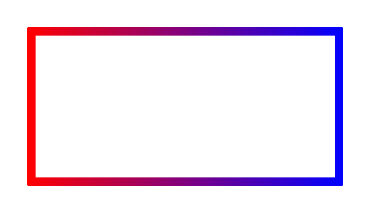
\begin{tikzpicture}
  \shade [left color=red,right color=blue] (-2,-1) rectangle (2,1);
  \begin{scope}[transparency group=knockout]
    \fill [white] (-1.9,-.9) rectangle (1.9,.9);
    \node [opacity=0,font=\fontencoding{T1}\fontfamily{ptm}\fontsize{45}{45}\bfseries]
          {Ti\emph{k}Z};
  \end{scope}
\end{tikzpicture}
\end{codeexample}
            %
            In the example, we first draw a large shading and then, inside the
            transparency group ``overwrite'' most of this shading by a big
            white rectangle. The interesting part is the text of the node,
            which has opacity |0|. Normally, this would mean that nothing is
            shown. However, in a knockout group, we ``paint'' the text with an
            ``opacity zero'' color. The effect is that part of the totally
            opaque white rectangle gets overwritten by a perfectly transparent
            area (namely exactly the area taken up by the pixels of the text).
            When this whole knockout group is then placed on top of the
            shading, the shading will ``shine through'' at the knocked-out
            pixels.

            在示例中,我们首先绘制了一个大的渐变,然后在透明度组内部通过一个大的白色矩形“覆盖”了大部分渐变。有趣的部分是节点的文本,其透明度为 |0|。通常,这意味着不会显示任何内容。然而,在 knockout 组中,我们使用“透明度为零”的颜色“绘制”文本。效果是,完全不透明的白色矩形的一部分被一个完全透明的区域覆盖(即正好是文本像素占据的区域)。当整个 knockout 组放置在渐变之上时,渐变将在被挖空的像素处“透过”。



        \item \declare{|isolated|}|=false| A group can be isolated or not. By
            default, they are isolated, since this is typically what you want.
            For details on what isolated groups are, exactly, see Section~7.3.4
            of the \textsc{pdf} Specification, version~1.7.

            \declare{|isolated|}|=false| 组可以是隔离的或非隔离的。默认情况下,它们是隔离的,因为这通常是您想要的。关于隔离组的详细信息,请参阅 \textsc{pdf} 规范版本 1.7 的第 7.3.4 节。


    \end{itemize}

    Note that when a transparency group is created, \tikzname\ must correctly
    determine the size of the material inside the group. Usually, this is no
    problem, but when you use things like |overlay| or |transform canvas|,
    trouble may result. In this case, please consult
    Section~\ref{section-transparency} on how to sidestep this problem in such
    cases.

    请注意,在创建透明度组时,\tikzname\ 必须正确确定组内部材料的大小。通常情况下,这没有问题,但是如果您使用了像 |overlay| 或 |transform canvas| 这样的东西,可能会出现问题。在这种情况下,请参阅第~\ref{section-transparency} 节以了解如何解决此类问题。


\end{key}


%%% Local Variables:
%%% mode: latex
%%% TeX-master: "pgfmanual"
%%% End:
